% =====================================================================
% Figure: Structural sensitivity matrix S_c on a toy ego-graph.
% Heatmap + leading right singular vector v_1.
%
% Data are loaded from paper/figures/data/{sc_heatmap_cells,sc_v1_bars}.tex
% which are auto-generated by scripts/build_figure_data.py. If those files
% are missing, scaffold values below take effect so the figure still
% compiles standalone.
%
% To use real numerics:
%   .venv/bin/python scripts/dump_sc_matrix_cora.py
%   .venv/bin/python scripts/build_figure_data.py
%   pdflatex paper/figures/fig_sc_heatmap.tex   # or rebuild aegis.pdf
%
% Standalone compile:
%   pdflatex -interaction=nonstopmode -halt-on-error fig_sc_heatmap.tex
% =====================================================================

\documentclass[tikz,border=4pt,11pt]{standalone}
\usepackage[T1]{fontenc}
\usepackage{mathptmx}
\usepackage{tikz}
\usepackage{xcolor}
\usepackage{amsmath, amssymb}
\usepackage{xspace}
\newcommand{\AEGIS}{\textsc{Aegis}\xspace}
\renewcommand{\familydefault}{\rmdefault}

\definecolor{caegis}{HTML}{009E73}
\definecolor{chigh}{HTML}{D55E00}

% Viridis-ish ramp mapping value in [0,1] -> colour
\newcommand{\heatcell}[3]{%
  \pgfmathsetmacro{\v}{#3}%
  \pgfmathsetmacro{\hue}{260 - 260*\v}%
  \pgfmathsetmacro{\sat}{55 + 35*\v}%
  \pgfmathsetmacro{\val}{30 + 65*\v}%
  \definecolor{cellc}{Hsb}{\hue,\sat,\val}%
  \fill[cellc] (#1*0.42, -#2*0.32) rectangle ++(0.42, -0.32);%
}

\begin{document}
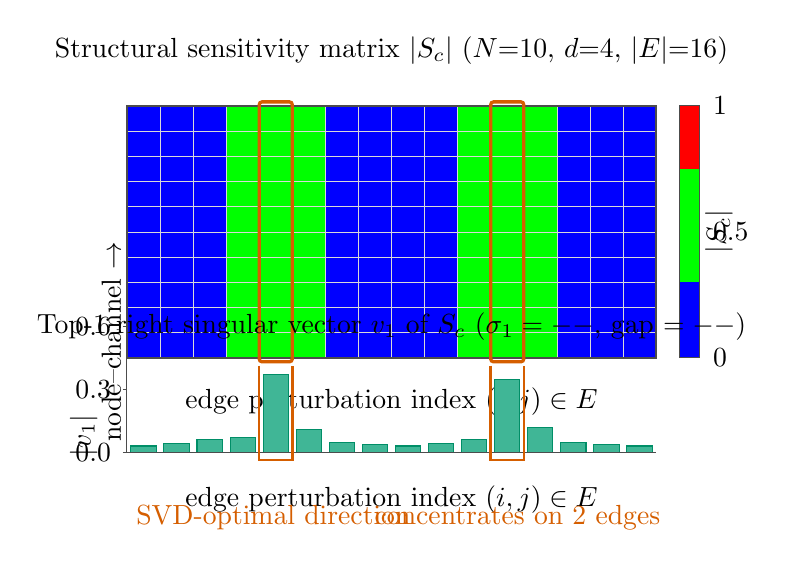
\begin{tikzpicture}[x=1cm,y=1cm]

% ---- Heatmap data (auto-generated if available; scaffold otherwise) ----
\IfFileExists{data/sc_heatmap_cells.tex}{%
  % AUTO-GENERATED by scripts/build_figure_data.py — do not edit by hand.
% Source: paper/figures/data/sc_matrix.npy  (downsampled 800x61 -> 14x28)
\def\schmRows{13}
\def\schmCols{27}

\heatcell{0}{0}{0.705}
\heatcell{1}{0}{0.762}
\heatcell{2}{0}{0.089}
\heatcell{3}{0}{0.064}
\heatcell{4}{0}{0.039}
\heatcell{5}{0}{0.083}
\heatcell{6}{0}{0.003}
\heatcell{7}{0}{0.002}
\heatcell{8}{0}{0.027}
\heatcell{9}{0}{0.059}
\heatcell{10}{0}{0.001}
\heatcell{11}{0}{0.050}
\heatcell{12}{0}{0.031}
\heatcell{13}{0}{0.025}
\heatcell{14}{0}{0.020}
\heatcell{15}{0}{0.048}
\heatcell{16}{0}{0.031}
\heatcell{17}{0}{0.050}
\heatcell{18}{0}{0.003}
\heatcell{19}{0}{0.052}
\heatcell{20}{0}{0.059}
\heatcell{21}{0}{0.058}
\heatcell{22}{0}{0.028}
\heatcell{23}{0}{0.028}
\heatcell{24}{0}{0.041}
\heatcell{25}{0}{0.051}
\heatcell{26}{0}{0.032}
\heatcell{27}{0}{0.042}
\heatcell{0}{1}{0.039}
\heatcell{1}{1}{0.062}
\heatcell{2}{1}{0.175}
\heatcell{3}{1}{0.738}
\heatcell{4}{1}{0.504}
\heatcell{5}{1}{0.144}
\heatcell{6}{1}{0.003}
\heatcell{7}{1}{0.002}
\heatcell{8}{1}{0.022}
\heatcell{9}{1}{0.061}
\heatcell{10}{1}{0.001}
\heatcell{11}{1}{0.041}
\heatcell{12}{1}{0.025}
\heatcell{13}{1}{0.020}
\heatcell{14}{1}{0.017}
\heatcell{15}{1}{0.040}
\heatcell{16}{1}{0.025}
\heatcell{17}{1}{0.041}
\heatcell{18}{1}{0.002}
\heatcell{19}{1}{0.041}
\heatcell{20}{1}{0.074}
\heatcell{21}{1}{0.047}
\heatcell{22}{1}{0.022}
\heatcell{23}{1}{0.023}
\heatcell{24}{1}{0.033}
\heatcell{25}{1}{0.046}
\heatcell{26}{1}{0.026}
\heatcell{27}{1}{0.035}
\heatcell{0}{2}{0.040}
\heatcell{1}{2}{0.065}
\heatcell{2}{2}{0.002}
\heatcell{3}{2}{0.055}
\heatcell{4}{2}{0.034}
\heatcell{5}{2}{0.688}
\heatcell{6}{2}{0.440}
\heatcell{7}{2}{0.147}
\heatcell{8}{2}{0.457}
\heatcell{9}{2}{0.169}
\heatcell{10}{2}{0.001}
\heatcell{11}{2}{0.043}
\heatcell{12}{2}{0.027}
\heatcell{13}{2}{0.020}
\heatcell{14}{2}{0.017}
\heatcell{15}{2}{0.041}
\heatcell{16}{2}{0.026}
\heatcell{17}{2}{0.042}
\heatcell{18}{2}{0.003}
\heatcell{19}{2}{0.044}
\heatcell{20}{2}{0.036}
\heatcell{21}{2}{0.049}
\heatcell{22}{2}{0.023}
\heatcell{23}{2}{0.024}
\heatcell{24}{2}{0.035}
\heatcell{25}{2}{0.041}
\heatcell{26}{2}{0.027}
\heatcell{27}{2}{0.036}
\heatcell{0}{3}{0.048}
\heatcell{1}{3}{0.074}
\heatcell{2}{3}{0.002}
\heatcell{3}{3}{0.064}
\heatcell{4}{3}{0.040}
\heatcell{5}{3}{0.353}
\heatcell{6}{3}{0.003}
\heatcell{7}{3}{0.076}
\heatcell{8}{3}{0.272}
\heatcell{9}{3}{0.842}
\heatcell{10}{3}{0.025}
\heatcell{11}{3}{0.049}
\heatcell{12}{3}{0.030}
\heatcell{13}{3}{0.029}
\heatcell{14}{3}{0.020}
\heatcell{15}{3}{0.049}
\heatcell{16}{3}{0.030}
\heatcell{17}{3}{0.050}
\heatcell{18}{3}{0.003}
\heatcell{19}{3}{0.050}
\heatcell{20}{3}{0.041}
\heatcell{21}{3}{0.058}
\heatcell{22}{3}{0.031}
\heatcell{23}{3}{0.028}
\heatcell{24}{3}{0.040}
\heatcell{25}{3}{0.048}
\heatcell{26}{3}{0.031}
\heatcell{27}{3}{0.042}
\heatcell{0}{4}{0.039}
\heatcell{1}{4}{0.062}
\heatcell{2}{4}{0.002}
\heatcell{3}{4}{0.052}
\heatcell{4}{4}{0.033}
\heatcell{5}{4}{0.068}
\heatcell{6}{4}{0.003}
\heatcell{7}{4}{0.002}
\heatcell{8}{4}{0.022}
\heatcell{9}{4}{0.048}
\heatcell{10}{4}{0.125}
\heatcell{11}{4}{0.701}
\heatcell{12}{4}{0.559}
\heatcell{13}{4}{0.021}
\heatcell{14}{4}{0.017}
\heatcell{15}{4}{0.039}
\heatcell{16}{4}{0.025}
\heatcell{17}{4}{0.040}
\heatcell{18}{4}{0.003}
\heatcell{19}{4}{0.042}
\heatcell{20}{4}{0.034}
\heatcell{21}{4}{0.048}
\heatcell{22}{4}{0.023}
\heatcell{23}{4}{0.023}
\heatcell{24}{4}{0.033}
\heatcell{25}{4}{0.039}
\heatcell{26}{4}{0.026}
\heatcell{27}{4}{0.034}
\heatcell{0}{5}{0.052}
\heatcell{1}{5}{0.072}
\heatcell{2}{5}{0.002}
\heatcell{3}{5}{0.061}
\heatcell{4}{5}{0.039}
\heatcell{5}{5}{0.080}
\heatcell{6}{5}{0.003}
\heatcell{7}{5}{0.232}
\heatcell{8}{5}{0.132}
\heatcell{9}{5}{0.056}
\heatcell{10}{5}{0.001}
\heatcell{11}{5}{0.048}
\heatcell{12}{5}{0.201}
\heatcell{13}{5}{0.817}
\heatcell{14}{5}{0.020}
\heatcell{15}{5}{0.048}
\heatcell{16}{5}{0.030}
\heatcell{17}{5}{0.050}
\heatcell{18}{5}{0.003}
\heatcell{19}{5}{0.049}
\heatcell{20}{5}{0.039}
\heatcell{21}{5}{0.062}
\heatcell{22}{5}{0.032}
\heatcell{23}{5}{0.028}
\heatcell{24}{5}{0.041}
\heatcell{25}{5}{0.047}
\heatcell{26}{5}{0.030}
\heatcell{27}{5}{0.041}
\heatcell{0}{6}{0.057}
\heatcell{1}{6}{0.088}
\heatcell{2}{6}{0.003}
\heatcell{3}{6}{0.075}
\heatcell{4}{6}{0.046}
\heatcell{5}{6}{0.097}
\heatcell{6}{6}{0.004}
\heatcell{7}{6}{0.002}
\heatcell{8}{6}{0.032}
\heatcell{9}{6}{0.069}
\heatcell{10}{6}{0.002}
\heatcell{11}{6}{0.058}
\heatcell{12}{6}{0.037}
\heatcell{13}{6}{0.031}
\heatcell{14}{6}{0.682}
\heatcell{15}{6}{0.821}
\heatcell{16}{6}{0.036}
\heatcell{17}{6}{0.058}
\heatcell{18}{6}{0.004}
\heatcell{19}{6}{0.060}
\heatcell{20}{6}{0.048}
\heatcell{21}{6}{0.305}
\heatcell{22}{6}{0.033}
\heatcell{23}{6}{0.033}
\heatcell{24}{6}{0.048}
\heatcell{25}{6}{0.056}
\heatcell{26}{6}{0.037}
\heatcell{27}{6}{0.049}
\heatcell{0}{7}{0.034}
\heatcell{1}{7}{0.049}
\heatcell{2}{7}{0.002}
\heatcell{3}{7}{0.042}
\heatcell{4}{7}{0.026}
\heatcell{5}{7}{0.054}
\heatcell{6}{7}{0.002}
\heatcell{7}{7}{0.015}
\heatcell{8}{7}{0.067}
\heatcell{9}{7}{0.038}
\heatcell{10}{7}{0.001}
\heatcell{11}{7}{0.032}
\heatcell{12}{7}{0.020}
\heatcell{13}{7}{0.020}
\heatcell{14}{7}{0.013}
\heatcell{15}{7}{0.033}
\heatcell{16}{7}{0.671}
\heatcell{17}{7}{0.673}
\heatcell{18}{7}{0.002}
\heatcell{19}{7}{0.033}
\heatcell{20}{7}{0.027}
\heatcell{21}{7}{0.040}
\heatcell{22}{7}{0.021}
\heatcell{23}{7}{0.019}
\heatcell{24}{7}{0.027}
\heatcell{25}{7}{0.032}
\heatcell{26}{7}{0.020}
\heatcell{27}{7}{0.028}
\heatcell{0}{8}{0.054}
\heatcell{1}{8}{0.084}
\heatcell{2}{8}{0.004}
\heatcell{3}{8}{0.071}
\heatcell{4}{8}{0.044}
\heatcell{5}{8}{0.092}
\heatcell{6}{8}{0.004}
\heatcell{7}{8}{0.002}
\heatcell{8}{8}{0.031}
\heatcell{9}{8}{0.066}
\heatcell{10}{8}{0.002}
\heatcell{11}{8}{0.056}
\heatcell{12}{8}{0.035}
\heatcell{13}{8}{0.029}
\heatcell{14}{8}{0.023}
\heatcell{15}{8}{0.054}
\heatcell{16}{8}{0.034}
\heatcell{17}{8}{0.055}
\heatcell{18}{8}{0.673}
\heatcell{19}{8}{0.886}
\heatcell{20}{8}{0.075}
\heatcell{21}{8}{0.065}
\heatcell{22}{8}{0.031}
\heatcell{23}{8}{0.031}
\heatcell{24}{8}{0.046}
\heatcell{25}{8}{0.058}
\heatcell{26}{8}{0.036}
\heatcell{27}{8}{0.047}
\heatcell{0}{9}{0.049}
\heatcell{1}{9}{0.073}
\heatcell{2}{9}{0.367}
\heatcell{3}{9}{0.062}
\heatcell{4}{9}{0.039}
\heatcell{5}{9}{0.081}
\heatcell{6}{9}{0.003}
\heatcell{7}{9}{0.002}
\heatcell{8}{9}{0.028}
\heatcell{9}{9}{0.057}
\heatcell{10}{9}{0.001}
\heatcell{11}{9}{0.048}
\heatcell{12}{9}{0.030}
\heatcell{13}{9}{0.027}
\heatcell{14}{9}{0.020}
\heatcell{15}{9}{0.290}
\heatcell{16}{9}{0.030}
\heatcell{17}{9}{0.049}
\heatcell{18}{9}{0.003}
\heatcell{19}{9}{0.049}
\heatcell{20}{9}{0.650}
\heatcell{21}{9}{1.000}
\heatcell{22}{9}{0.029}
\heatcell{23}{9}{0.028}
\heatcell{24}{9}{0.040}
\heatcell{25}{9}{0.144}
\heatcell{26}{9}{0.031}
\heatcell{27}{9}{0.041}
\heatcell{0}{10}{0.044}
\heatcell{1}{10}{0.063}
\heatcell{2}{10}{0.002}
\heatcell{3}{10}{0.054}
\heatcell{4}{10}{0.034}
\heatcell{5}{10}{0.070}
\heatcell{6}{10}{0.003}
\heatcell{7}{10}{0.002}
\heatcell{8}{10}{0.026}
\heatcell{9}{10}{0.049}
\heatcell{10}{10}{0.001}
\heatcell{11}{10}{0.041}
\heatcell{12}{10}{0.027}
\heatcell{13}{10}{0.026}
\heatcell{14}{10}{0.017}
\heatcell{15}{10}{0.042}
\heatcell{16}{10}{0.026}
\heatcell{17}{10}{0.044}
\heatcell{18}{10}{0.003}
\heatcell{19}{10}{0.042}
\heatcell{20}{10}{0.034}
\heatcell{21}{10}{0.053}
\heatcell{22}{10}{0.625}
\heatcell{23}{10}{0.108}
\heatcell{24}{10}{0.035}
\heatcell{25}{10}{0.041}
\heatcell{26}{10}{0.026}
\heatcell{27}{10}{0.036}
\heatcell{0}{11}{0.042}
\heatcell{1}{11}{0.064}
\heatcell{2}{11}{0.002}
\heatcell{3}{11}{0.054}
\heatcell{4}{11}{0.034}
\heatcell{5}{11}{0.070}
\heatcell{6}{11}{0.003}
\heatcell{7}{11}{0.002}
\heatcell{8}{11}{0.024}
\heatcell{9}{11}{0.050}
\heatcell{10}{11}{0.226}
\heatcell{11}{11}{0.042}
\heatcell{12}{11}{0.026}
\heatcell{13}{11}{0.023}
\heatcell{14}{11}{0.017}
\heatcell{15}{11}{0.041}
\heatcell{16}{11}{0.026}
\heatcell{17}{11}{0.043}
\heatcell{18}{11}{0.003}
\heatcell{19}{11}{0.044}
\heatcell{20}{11}{0.035}
\heatcell{21}{11}{0.051}
\heatcell{22}{11}{0.025}
\heatcell{23}{11}{0.733}
\heatcell{24}{11}{0.713}
\heatcell{25}{11}{0.041}
\heatcell{26}{11}{0.027}
\heatcell{27}{11}{0.036}
\heatcell{0}{12}{0.037}
\heatcell{1}{12}{0.057}
\heatcell{2}{12}{0.006}
\heatcell{3}{12}{0.048}
\heatcell{4}{12}{0.030}
\heatcell{5}{12}{0.063}
\heatcell{6}{12}{0.003}
\heatcell{7}{12}{0.002}
\heatcell{8}{12}{0.022}
\heatcell{9}{12}{0.044}
\heatcell{10}{12}{0.001}
\heatcell{11}{12}{0.038}
\heatcell{12}{12}{0.023}
\heatcell{13}{12}{0.022}
\heatcell{14}{12}{0.015}
\heatcell{15}{12}{0.037}
\heatcell{16}{12}{0.023}
\heatcell{17}{12}{0.038}
\heatcell{18}{12}{0.002}
\heatcell{19}{12}{0.039}
\heatcell{20}{12}{0.133}
\heatcell{21}{12}{0.045}
\heatcell{22}{12}{0.024}
\heatcell{23}{12}{0.022}
\heatcell{24}{12}{0.031}
\heatcell{25}{12}{0.731}
\heatcell{26}{12}{0.748}
\heatcell{27}{12}{0.032}
\heatcell{0}{13}{0.289}
\heatcell{1}{13}{0.405}
\heatcell{2}{13}{0.013}
\heatcell{3}{13}{0.353}
\heatcell{4}{13}{0.219}
\heatcell{5}{13}{0.453}
\heatcell{6}{13}{0.280}
\heatcell{7}{13}{0.011}
\heatcell{8}{13}{0.156}
\heatcell{9}{13}{0.311}
\heatcell{10}{13}{0.008}
\heatcell{11}{13}{0.263}
\heatcell{12}{13}{0.175}
\heatcell{13}{13}{0.172}
\heatcell{14}{13}{0.111}
\heatcell{15}{13}{0.263}
\heatcell{16}{13}{0.167}
\heatcell{17}{13}{0.277}
\heatcell{18}{13}{0.017}
\heatcell{19}{13}{0.277}
\heatcell{20}{13}{0.224}
\heatcell{21}{13}{0.358}
\heatcell{22}{13}{0.173}
\heatcell{23}{13}{0.155}
\heatcell{24}{13}{0.228}
\heatcell{25}{13}{0.266}
\heatcell{26}{13}{0.175}
\heatcell{27}{13}{0.931}
%
}{%
  % SCAFFOLD: 10 rows x 16 cols with dominant columns at 4 and 11.
  \def\schmRows{9}\def\schmCols{15}%
  \foreach \r in {0,...,9} {%
    \foreach \c in {0,...,15} {%
      \pgfmathparse{(\c == 4 || \c == 11) ? 0.80 + 0.05*sin(36*\r) :
                    (abs(\c-4) < 2 || abs(\c-11) < 2) ? 0.45 + 0.05*cos(45*\r) :
                    0.10 + 0.12*(rand+0.5)*0.4 + 0.04*sin(18*(\r+\c))}%
      \edef\val{\pgfmathresult}%
      \heatcell{\c}{\r}{\val}%
    }%
  }%
}

% Compute axis extents from the data-provided counts
\pgfmathsetmacro{\axW}{(\schmCols+1)*0.42}
\pgfmathsetmacro{\axH}{(\schmRows+1)*0.32}

% ---- Grid lines for readability ----
\foreach \c in {0,...,99} {%
  \ifnum\c>\schmCols\else
    \pgfmathsetmacro{\xc}{\c*0.42}%
    \draw[gray!30, line width=0.2pt] (\xc, 0.0) -- (\xc, -\axH);%
  \fi
}
\pgfmathsetmacro{\xcR}{(\schmCols+1)*0.42}
\draw[gray!30, line width=0.2pt] (\xcR, 0.0) -- (\xcR, -\axH);
\foreach \r in {0,...,99} {%
  \ifnum\r>\schmRows\else
    \pgfmathsetmacro{\yr}{-\r*0.32}%
    \draw[gray!30, line width=0.2pt] (0, \yr) -- (\axW, \yr);%
  \fi
}
\pgfmathsetmacro{\yrB}{-(\schmRows+1)*0.32}
\draw[gray!30, line width=0.2pt] (0, \yrB) -- (\axW, \yrB);

% Border
\draw[black!70, line width=0.5pt] (0,0) rectangle (\axW, -\axH);

% ---- v_1 data (defines \vonelist, \voneCount, \voneHighA, \voneHighB) ----
\IfFileExists{data/sc_v1_bars.tex}{%
  % AUTO-GENERATED by scripts/build_figure_data.py — do not edit by hand.
% Source: paper/figures/data/sc_v1.npy  (61 edges; sampled to 28 for display)
\def\vonelist{{0.482, 0.788, 0.088, 0.685, 0.395, 1.000, 0.122, 0.054, 0.304, 0.742, 0.039, 0.518, 0.337, 0.282, 0.234, 0.619, 0.335, 0.510, 0.100, 0.556, 0.473, 0.763, 0.272, 0.347, 0.423, 0.541, 0.346, 0.454}}
\def\voneCount{27}
\def\voneHighA{5}
\def\voneHighB{1}
\newcommand{\schmTopThreeMass}{0.22}
%
}{%
  \def\vonelist{{0.05, 0.07, 0.10, 0.12, 0.62, 0.18, 0.08, 0.06, 0.05, 0.07, 0.10, 0.58, 0.20, 0.08, 0.06, 0.05}}%
  \def\voneCount{15}%
  \def\voneHighA{4}%
  \def\voneHighB{11}%
}

% Highlight dominant columns (from v_1)
\pgfmathsetmacro{\hAx}{\voneHighA*0.42}
\pgfmathsetmacro{\hAxR}{(\voneHighA+1)*0.42}
\pgfmathsetmacro{\hBx}{\voneHighB*0.42}
\pgfmathsetmacro{\hBxR}{(\voneHighB+1)*0.42}
\draw[chigh, line width=1.2pt, rounded corners=1pt]
  (\hAx, 0.05) rectangle (\hAxR, -\axH - 0.05);
\draw[chigh, line width=1.2pt, rounded corners=1pt]
  (\hBx, 0.05) rectangle (\hBxR, -\axH - 0.05);

% ---- Axis labels (use meta if available) ----
\IfFileExists{data/sc_meta.tex}{%
  % AUTO-GENERATED by scripts/build_figure_data.py — do not edit by hand.
\newcommand{\schmN}{50}
\newcommand{\schmDim}{16}
\newcommand{\schmEdges}{61}
\newcommand{\schmSigmaOne}{41.185}
\newcommand{\schmGap}{0.43}
%
}{%
  \newcommand{\schmN}{10}%
  \newcommand{\schmDim}{4}%
  \newcommand{\schmEdges}{16}%
  \newcommand{\schmSigmaOne}{--}%
  \newcommand{\schmGap}{--}%
}

\pgfmathsetmacro{\axMid}{\axW/2}
\node[font=\normalsize, anchor=south] at (\axMid, 0.4)
  {Structural sensitivity matrix $|S_c|$ ($N{=}\schmN$, $d{=}\schmDim$, $|E|{=}\schmEdges$)};
\node[font=\normalsize, anchor=east, rotate=90] at (-0.2, -\axH/2) {node--channel $\to$};
\node[font=\normalsize, anchor=north] at (\axMid, -\axH - 0.25)
  {edge perturbation index $(i,j) \in E$};

% ---- Colorbar (vertical, right side) ----
\pgfmathsetmacro{\cbX}{\axW + 0.30}
\pgfmathsetmacro{\cbXR}{\axW + 0.55}
\pgfmathsetmacro{\cbStep}{\axH/20}
\foreach \i in {0,...,19} {%
  \pgfmathsetmacro{\vv}{\i/19}%
  \pgfmathsetmacro{\hue}{260 - 260*\vv}%
  \pgfmathsetmacro{\sat}{55 + 35*\vv}%
  \pgfmathsetmacro{\val}{30 + 65*\vv}%
  \definecolor{cbc}{Hsb}{\hue,\sat,\val}%
  \pgfmathsetmacro{\ybot}{-\axH + \i*\cbStep}%
  \pgfmathsetmacro{\ytop}{-\axH + (\i+1)*\cbStep}%
  \fill[cbc] (\cbX, \ybot) rectangle (\cbXR, \ytop);%
}
\draw[black!70, line width=0.4pt] (\cbX, -\axH) rectangle (\cbXR, 0);
\node[font=\normalsize, anchor=west] at (\cbXR + 0.05, -\axH) {0};
\node[font=\normalsize, anchor=west] at (\cbXR + 0.05, -\axH/2) {0.5};
\node[font=\normalsize, anchor=west] at (\cbXR + 0.05, 0) {1};
\node[font=\normalsize, rotate=90, anchor=south] at (\cbXR + 0.55, -\axH/2) {$|S_c|$};

% ---- Bottom panel: v_1 bars ----
\pgfmathsetmacro{\vshift}{-\axH - 1.2}
\begin{scope}[shift={(0, \vshift)}]
  \foreach \c in {0,...,99} {%
    \ifnum\c>\voneCount\else
      \pgfmathparse{\vonelist[\c]}%
      \pgfmathsetmacro{\bh}{\pgfmathresult * 1.6}%
      \fill[caegis!75, draw=caegis!90!black]
        (\c*0.42 + 0.05, 0) rectangle ++(0.32, \bh);%
    \fi
  }%

  % Axis line
  \draw[black!70, line width=0.4pt] (0, 0) -- (\axW, 0);
  \draw[black!70, line width=0.4pt] (0, 0) -- (0, 1.2);
  \foreach \y/\lab in {0.0/0.0, 0.5/0.3, 1.0/0.6} {%
    \pgfmathsetmacro{\yp}{\y * 1.6}%
    \draw[black!70, line width=0.3pt] (-0.05, \yp) -- (0, \yp);%
    \node[font=\normalsize, anchor=east] at (-0.08, \yp) {\lab};%
  }

  % Highlight top-2
  \pgfmathsetmacro{\xA}{\voneHighA*0.42}
  \pgfmathsetmacro{\xAR}{(\voneHighA+1)*0.42}
  \pgfmathsetmacro{\xB}{\voneHighB*0.42}
  \pgfmathsetmacro{\xBR}{(\voneHighB+1)*0.42}
  \draw[chigh, line width=0.9pt]
    (\xA, 1.10) -- (\xA, -0.10) -- (\xAR, -0.10) -- (\xAR, 1.10);
  \draw[chigh, line width=0.9pt]
    (\xB, 1.10) -- (\xB, -0.10) -- (\xBR, -0.10) -- (\xBR, 1.10);

  \node[font=\normalsize, anchor=south] at (\axMid, 1.30)
    {Top-1 right singular vector $v_1$ of $S_c$ ($\sigma_1 = \schmSigmaOne$, gap $= \schmGap$)};
  \node[font=\normalsize, anchor=north] at (\axMid, -0.30)
    {edge perturbation index $(i,j) \in E$};
  \node[font=\normalsize, anchor=east, rotate=90] at (-0.55, 0.6) {$|v_1|$};

  \node[font=\normalsize, color=chigh, anchor=north] at (\axMid - 1.5, -0.55)
    {SVD-optimal direction};
  \node[font=\normalsize, color=chigh, anchor=north] at (\axMid + 1.6, -0.55)
    {concentrates on 2 edges};
\end{scope}

\end{tikzpicture}
\end{document}
